\ts\space is a material in the group of \acp{TMD}.
All \ac{TMD} appear in the general form MX\textsubscript{2} with M being a layer of transition-metal atoms such as molybdenum, tungsten or titanium which are sitting between two layers of species X from the group of chalcogens like sulfur or selenium.
This covalently bonded structure is called a \ac{TMD} monolayer.
\Ac{TMD} bulk material is made up of many monolayers stacked monolayers, bonded by van-der-Waals interaction.

The research part of my studies will focus on the \ac{TMD} \textit{1T}-\ts, the \textit{1T}-prefix is referring to the stacking order of the monolayers, that results in octahedrally coordinated titanium atoms.
From here on out it will simply be referred to as \ts.
Its crystal structure at room temperature and atmospheric pressure is depicted in figure~\ref{fig:crystal}\,a.
The unit cell contains one Ti atom and two Se atoms and the lattice vectors have lengths of $\mathbf{a}=\mathbf{b}=3.541$\,\AA\space and $\mathbf{c}=6.001$\,\AA\cite{patel1983}.

\begin{figure}[!t]
	\begin{minipage}{0.5\columnwidth}
		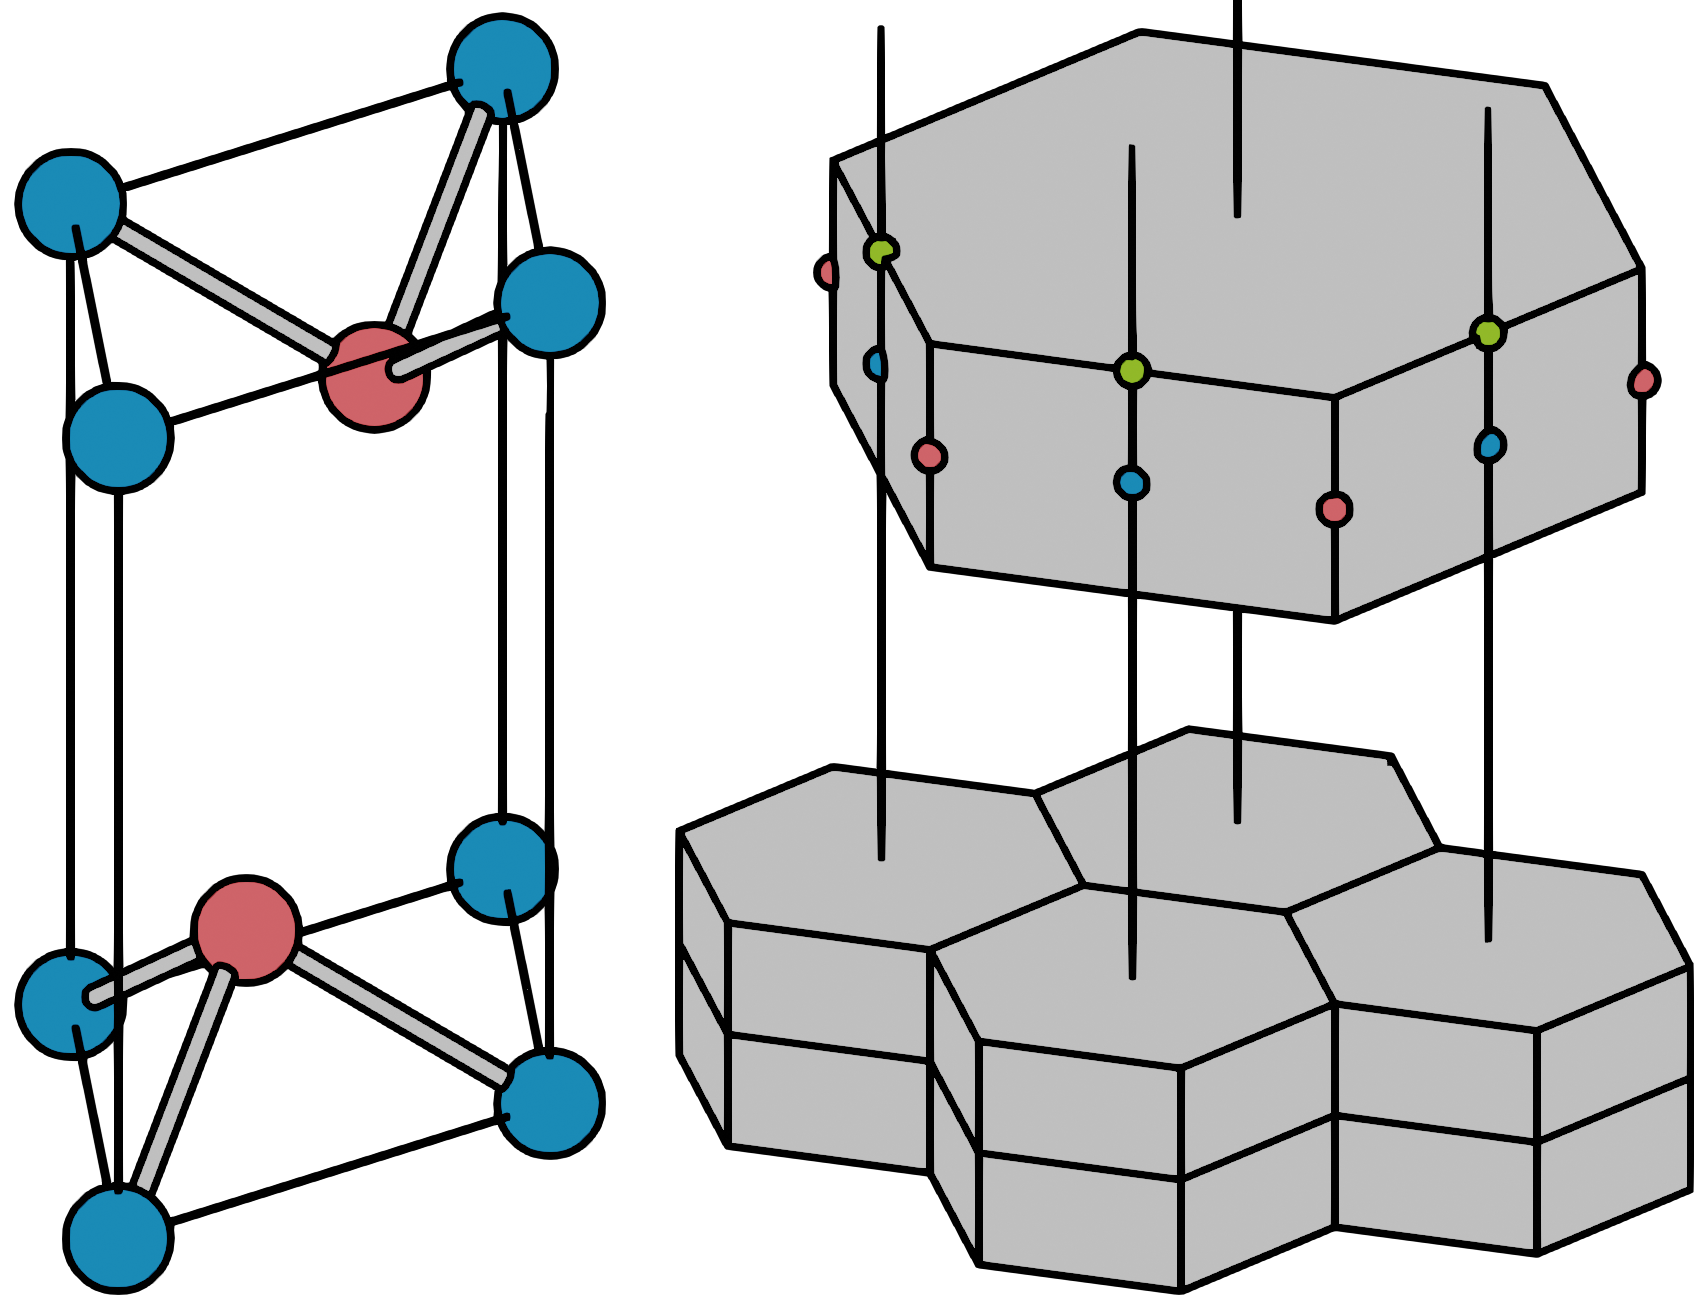
\includegraphics[width=\columnwidth]{figs/tise2_crystal.png}
	\end{minipage}
	\hspace{0.04\columnwidth}
	\begin{minipage}{0.45\columnwidth}
		\caption{a)\,Hexagonal unit cell of \ts, comprised of one Ti atom and two Se atoms. Ti atoms are shown in blue, Se atoms in red. b)\,\ac{BZ} of the high temperature phase (top) and low temperature phase (bottom) of \ts. Blue/red spheres mark M/L points in the \ac{BZ}}
		\label{fig:crystal}
	\end{minipage}
\end{figure}

The material shows semi-metallic electronic characteristics\cite{bachrach1976}, with a hole pocket from the Se 4s band at the $\Gamma$ point of the \ac{BZ} and an electron pocket at the L point from the Ti 3d band\cite{zunger1978}.

Upon cooling, at 200\,K \cite{disalvo1976} \ts\space undergoes a second order phase transition into a phase with a commensurate 2$\times$2$\times$2 \ac{PLD} accompanied by a \ac{CDW} \cite{rossnagel2011}.
\ac{CDW} and \ac{PLD} go hand in hand, since a periodic modulation of the electron density will shift the equilibrium positions of the ions.
Vice versa, periodically displaced ions will alter the electron density to more adequately screen their potential.
Currently two mechanisms are discussed to drive the transition: 
firstly, the band Jahn-Teller effect describing the splitting of two degenerate energy bands due broken symmetry introduced by structural changes\cite{JT}.
Secondly, the formation of a excitonic insulator ground state due to cooperative interaction between the charge carriers\cite{EI}.
